\chapter[Voltage unbalance compensation]{Voltage unbalance compensation with geometrical indicator on a domestic low voltage network}\label{BASIC:sec:unbalance_compensation}

\section{Literature overview}
%============ Network properties and uncertainties
% MonteCarlo
\hlc[MA]{The phenomena of voltage unbalance (VU)}\hlc[PT]{ was investigated for a long time. VU of three-phase voltages results from asymmetry of line impedances and from inequality of loads in three phase networks. Efforts are in general are made to reduce the asymmetry, sprouting form network topology geometries impedance by transposition. On the other hand, voltage unbalance caused by uneven distribution of loads over three phases is more difficult to compensate. In low voltage residential and/or commercial systems, single-phase loads account for the majority of power consumption. Wherever possible,efforts are made to distribute the single phase loads uniformly over three phases, but residential areas are generally not sanctioned per household. It is unlikely that at a given instant loads in the three phases are balanced because they vary in a random manner. In other words, even if the average loads in the three phases are kept the same, the instantaneous power demands in the three phases differ from each other, leading to unbalanced voltages at the point of common coupling. With this in mind, predictive models can not reliably established, however stochastic models has been tried to aid the effort. In} \cite{wang2001method}\hlc[PT]{ a distribution networks were examined, and a Monte Carlo analysis with random variation of the voltage unbalance factor is modeled with the aid of correlated Gaussian random variables that represent random variations in three-phase active and reactive powers. Also this method used in} \cite{schwanz2016stochastic} and \cite{schwanz2016stochastic}, \hlc[PT]{for single phase power plants (mainly PV plants) caused VU risk assessment and mitigation. It was shown that this unchecked plants can cause serious risk with above $2\%$ VUF, and the maximum single-phase and uncontrolled connection of plants is unacceptably high, posing a risk for other networks as well.}\\
% Covariance + neural
\hlc[PT]{The authors of }\cite{xu2018stochastic}\hlc[PT]{ proposed a stochastic multi-objective optimization to model VU, where the discrete decision variables are coordinated with continuous regulation of solar reactive outputs updating they assumed covariances. For the purpose, the stochastic processes of solar active power are modelled in a scenario based framework. Stochastic processes were converted into a series of equivalent deterministic scenarios. For this purpose, a modified non-dominated sorting genetic algorithm-II was proposed, in which crossover rate and mutation rate are dynamically revised by a fuzzy logic controller.}\\
%============ UNBALANCE COMPENSATION
\hlc[PT]{There are different approaches of lowering the unbalance with different control techniques. Since conventional inverter topologies ar built for symmetrical, and zero offset current and voltage waveforms, the topology needed to change, to compensate the negative (and occasionally zero) sequence symmetrical components, besides normal operation. An interesting approach by} \cite{li2005microgrid} \hlc[PT]{was introduced, where two parallel VSIs are connected to produce positive and negative sequence components side by side. The approach also utilizes optimal control to achieve both the quality of power (MPPT) within the microgrid and the quality of currents (unbalance mitigation with low THD) flowing between the microgrid and the utility system, where two parts are controlled complementarily to inject negative- and zero-sequence currents in series to balance the line currents, while
generating zero real and reactive power. An other approach, is to try to estimate the required compensation geometrically by} \cite{lee2009new}, \hlc[PT]{where the required step in space vector modulation (SVM) is calculated by giving the assumed vectorial sum to move the measured system to a more balanced state. The authors use a series connected VSI (with common DC link) to achieve the required freedom for the operation, although the unbalance reduction is for the controlled three phase loads only, and the network is not influenced.\\
In the market there are devices with the sole purpose of compensation, and one of them is the static var compensator (SVC). This device is connected parallel, to the network (usually after the transformer station) to adaptively reduce the networks reactive power. However in} \cite{xu2010voltage} \hlc[PT]{the SVC is used also for mitigating the grid's VU. In the article, as three-phase IGBT-based static synchronous compensator was proposed for voltage and/or current unbalance compensation, where an instantaneous power theory (IPT) was used for real-time calculation and control. This control approach calculates the controller's next step from the instantaneous values of voltage and current to formulate the required power to inject in an averaged time interval.\\
In some cases the authors aim not to reduce the effect of unbalance on the network, but to ensure stable operation, while devices and loads are protected. In} \cite{vekhande2015control} \hlc[PT]{the authors argue, that working under network VU, a current source inverter (CSI) holds a better strategy, than its counterpart, although the device is only operates under this condition and does not contribute to the unbalance even further. The device stands as gateway between a DC microgrid and an AC grid. Under the effect of VU the DC microgrid suffers harmonic oscillations in voltage, and possible controller tripping (one phase exceeds the current limit) if it is not mitigated. The authors mention the use of conventional VSI based structures for CSI may lead to unstable operation, as such, they inject balanced three phase currents into the AC grid under an unbalanced grid voltage. Based on the instantaneous active power theory under unbalanced  grid conditions} \cite{wang2016dc} \hlc[PT]{proposes an optimized negative-sequence current references for  eliminating the double-frequency oscillations on active power at AC side of a current source converter. The approach is similar as before, using CSI as a good topology candidate, as well as the control structure of IPT, but the goal here is also to work under unbalanced grid conditions, and only protecting the device and the load. In} \cite{guo2018advanced} \hlc[PT]{direct control strategy with CSI model based control is shown which is simpler than the complicated IPT. The factors of unbalance are measured (negative and zero sequence as well) and the optimal current is calculated from the device model and from the factors via phase locked loop.\\
As an issue both} {\cite{Hu2016264}, and \cite{el2016control} \hlc[PT]{names the increasing PV penetration a thread for the network quality, namely the voltage balance. The former suggests that the network operators are  mainly obligated to mitigate the phenomena, by the transmission systems management and control, and the former suggests a local strategy. The idea is to use the PV-VSI (voltage source inver with photovoltaic source on the DC end) as the control reserve for VU mitigation. Here also geometrical approach is used with SVI to calculate the VSI's next step and formulate the optimal voltage vector on the voltage phasor, and an intermediate PI controller to reduce parameter sensitivity. The controller's cost function is derived via current and voltage measurement based on the IPT.\\
In this dissertation the approach is, that the low voltage network's level of unbalance only depends on the habits of household residents, as such it is assumed, that the network beyond the connection point is unknown (the amount, type and power of domestic loads are unknown), and network impedance's stochastic distribution function can not be estimated as it shall be discussed in section }\oldref{VUB:sec:Statement}\hlc[PT]{. This implies, that the compensation's goal is to find the local optimum regardless of unknown conditions. Furthermore, the goal is to compensate the VU, without the option to place current controllers after the connection point. This implies, that the grid's transformer's current can not be measured, to esteem the network's behaviour. With this in mind,} in section \oldref{VUB:sec:Optimization} \hlc[PT]{ a control strategy was chosen, which was adequate for said conditions, and searches for the optimum without the necessity of knowing the control gradients. The authors in }\cite{dash2011dynamic} \hlc[PT]{suggest, that current control strategies, where non harmonic currents were used deemed to have difficulties, however the CSI exhibits higher reliability and power density than the VSC with added DC-DC boost converter topology. As such a current source based strategy with only harmonic currents were used, which shall be presented in section} \oldref{VUB:sec:Inverter}.
%%
%Additionally, new computationally efficient control techniques have been presented by \cite{lee2009new} to estimate and compensate input voltage unbalance (VU) disturbances for a voltage source converter. These tools are designed to be effective with high power systems with slower PWM switching frequencies of 5 kHz or lower and limited current-controller bandwidth. About the unbalance compensation control aspect, a three-phase IGBT-based static synchronous compensator were proposed for voltage and/or current unbalance compensation by \cite{xu2010voltage}. An instantaneous power theory was used for real-time calculation and control. Three control schemes current control, voltage control and integrated control were proposed to compensate unbalanced voltage, unbalanced current or both. Unbalance phenomena and power quality can be examined with modeling too. A particular modeling method was presented by \cite{li2005microgrid}, where a three-phase four-wire grid-interfacing power quality compensator were modeled. During voltage unbalance, the compensator, used a shunt with a series four phase inverter, could enhance both the quality of power within the microgrid and the quality of currents flowing between the microgrid and utility system. In this case a microgrid is a group of interconnected loads and distributed energy resources within clearly defined electrical boundaries that acts as a single controllable entity with respect to the grid. A microgrid can connect and disconnect from the grid to enable it to operate in both grid-connected or island-mode. The shunt four-leg inverter were controlled to maintain a set of balanced distortion free voltages to regulate power sharing among the parallel-connected distributed generation systems. Simulation studies were carried out by \cite{Hu2016264} where one of the aims was to develop and test the feasibility of a decoupled three-phase on-load tap charger in the distribution system with the objective of improving the distribution network power quality. Further control methods were applied for the solution for balancing of the most sensitive with regard to electric energy quality part of power system by \cite{korovkin2016uimethod}, minimizing the active power losses, stabilization of three-phase voltages, enhancement of asynchronous machine performance stability and reduction of errors occurring in power consumption measuring circuits.\\
%%============ UNBALANCE COMPENSATION WITH OF CURRENT SOURCE CONVERTERS
%In the arsenal of voltage unbalance compensation, current source power electronic devices have a dedicated position. Based on the instantaneous active power theory under unbalanced  grid conditions \cite{wang2016dc} proposes an optimized negative-sequence current  references  for  eliminating  the double-frequency  oscillations  on  active  power  at  AC  side of a current source converter. The author argues in \cite{wang2014virtual} that a classification of the virtual impedances can greatly benefit an unbalance compensating control structure, with an active stabilization method. In \cite{guo2018advanced} direct control strategy with detailed current converter model is shown which is much simpler than the complicated instantaneous power theory approach. This solution needs less voltage and current sensors for the feedback control, which means that it is a cost-effective solution. An interesting, yet similar approach compared in the paper if a bi-directional current source topology is used like in \cite{vekhande2015control}. This enables to compensate a much larger degree of freedom handing unbalanced conditions with the precaution of unstable operation possibilities.\\

\section{Power electronic components for current control}\label{BASICCSR:sec:PowerGeneral}

As the introduction suggest the main topic of the thesis is optimal current control. As such for reaching the desired optimum, the necessary actuators are needed for the task. For this, power electric converters are used, all of them based on a simple principle, namely they use controllable switches to set the required voltage level or the conducting current value, required on the load's end.


\subsection{Galvanic decoupled bi-directional DC-DC converters}\label{BASICCSR:sec:DCDC}

In this section a basic galvanic decoupled voltage source DC-DC converter shall be presented. In many DC power supplies, a galvanic isolation between the DC or AC input and the DC output is required for safety and reliability. An economical mean of achieving such an isolation is to employ a transformer version of a DC-DC converter. High-frequency transformers are of small size and weight and provide high efficiency. Their turns ratio can be used to additionally adjust the output voltage level. Generally, electric power generated by renewable energy sources is unstable in nature, thus producing an unwanted effect on the utility grid. This fact motivates research on energy storage and quality systems to smooth out active-power flow.\\
On the converter Fig.\ref{BASICCSR:fig:DCDCGalvanic} has two symmetrical single-phase voltage-source full-bridge converters, allowing a bi-directional power flow. Thanks to advancement in power device technology over the last decade the DC-DC devices are able to operate at an efficiency as high as $\approx97\%$ by using the latest trench-gate IGBTs. Therefore this topology has become a promising candidate as a power electronic interface for an energy storage and renewable system \cite{kheraluwala1992performance} \cite{inoue2007bidirectional}.


\begin{figure}[!ht]
        \centering
        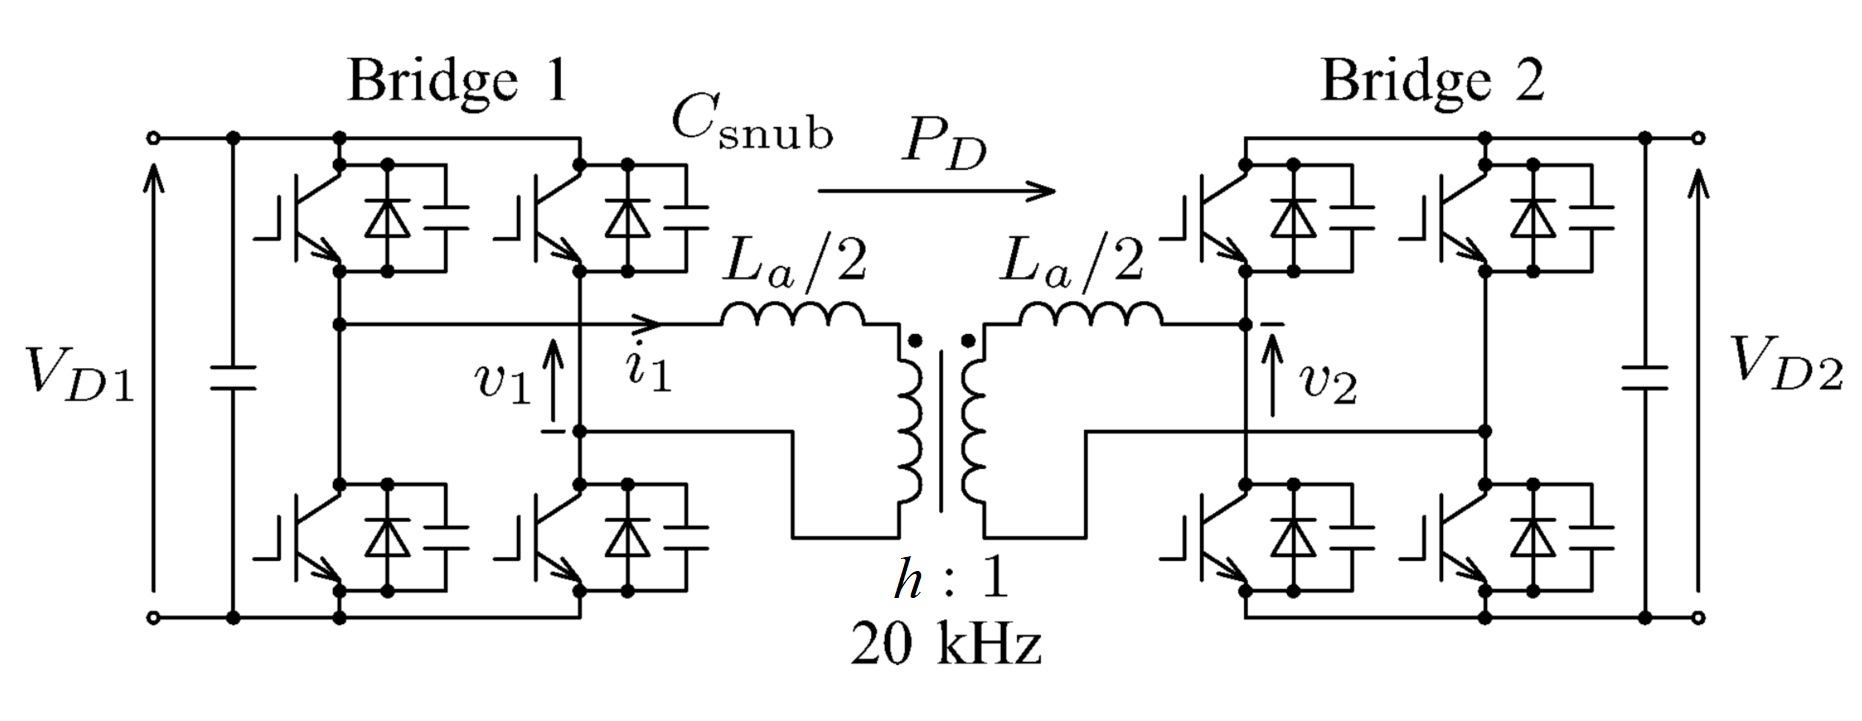
\includegraphics[width=0.7\textwidth]{EMPC_PNG_Pics/DC_DC_galvanic.png}
        \caption{Bidirectional isolated DC-DC converter, where $V_{D1}$, and $V_{D2}$ are the two end's voltage (in- and output depends on the power flow), $v_1$ and $v_2$ are the transformer voltages, $C_{snub}$ are to reduce switching loss and to damp out
over-voltage, and $h$ is the transformer turn ratio.}
        \label{BASICCSR:fig:DCDCGalvanic}
    \end{figure}
		
The principle of operation of the DC-DC converter is very simple. Two active bridges are interfaced through a transformer and are phase shifted from each other to control the amount of power flow from one DC voltage source to the other. This allows a fixed frequency, square-wave mode of operation and utilization of the leakage inductance of the transformer as the main energy transfer element. The power transfer under idealized conditions is defined as:

\begin{equation}
        \begin{array}{rcl}
            P_D&=&\frac{V_{D1}V_{D2}}{\omega L_a}\left(\delta-\frac{\delta^2}{\pi}\right)\\
        \end{array}
        \label{BASICMPC:equ:DCDC}
    \end{equation}
		
		where $\omega=2\pi f$ is the switching angular frequency of the two single phase full bridge controllers, $L_a$ is the
sum of the transformer leakage inductance.

\subsection{Current source inverters}\label{BASICCSR:sec:CSI}

Single-phase inverter's operating principles are different in each converter. The main features of the different approaches are reviewed and presented in the following. Although these converters cover the low-power range, they are widely used in power supplies or single-phase supplies. For this thesis a domestic current source inverter is considered, which fits into this category.\\
A current source inverter is composed of capacitors, switches, and diodes, where an array of two switches is called inverter leg shown in Fig.\ref{BASICCSR:fig:SingleCSI}. The capacitors required to provide a neutral point, such that each capacitor maintains a constant voltage.

\begin{figure}[!ht]
        \centering
        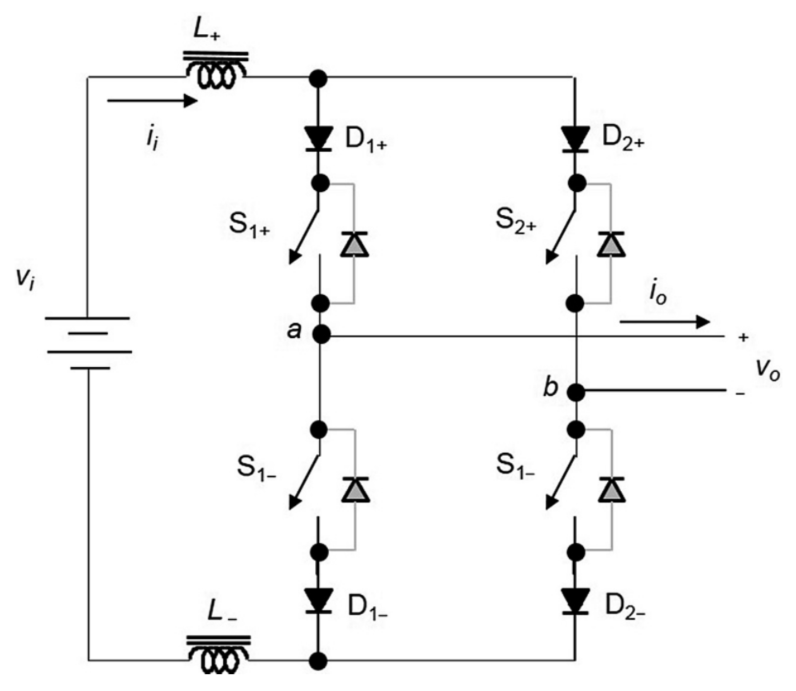
\includegraphics[width=0.6\textwidth]{EMPC_PNG_Pics/CurrentSourceInverter.png}
        \caption{Topology of a singly phase current source inverter, where $V_i$, and $V_o$ are the input and output voltages, $i_i$, and $i_o$ are the input and output currents respectively. $L_+$ and $L_-$ are current filter inductances, $S_{1+}$, $S_{2+}$, $D_{1+}$, and $D_{2+}$ are the higher switches (controlled IGBTs for instance) and diodes, and $S_{1-}$, $S_{2-}$, $D_{1-}$, and $D_{2-}$ are the lower switches and diodes respectively.}
        \label{BASICCSR:fig:SingleCSI}
    \end{figure}

The inductors required are large, such that the inductors
maintain a constant current $i_i$. Current-source topologies feature a low switching voltage gradient and reliable over-current or short-circuit protection. In order to operate properly the current-source inverter, we need to adhere to the following rules:
\begin{itemize}
\item Top or bottom switches of the different legs cannot be off simultaneously, because no current path is provided to the input inductors.
\item Diode must be placed in series with each switch, because a short circuit across the output voltage $V_o$ would be produced. If the commercial switch does not include anti- parallel diodes, then the circuit is already complete.
\item In practical implementation, an overlapping time must be considered in the control signals of the top or bottom switches of the different legs.
\end{itemize}

According to the previous rules, it should be noticed that all switches of the inverter leg can be turned on at the same time. This is not possible in voltage source inverters. There are four ($1^{st}$ to $4^{th}$) defined states of the switches and one not permitted switching state ($5^{th}$ state) as shown in Table \ref{BASICCSR:table:CSIstates}. The modulating technique should always ensure that at any instant, at least one of the top and bottom switch of the inverter legs is on, otherwise the inverter will be damaged.

% Please add the following required packages to your document preamble:
% \usepackage{multirow}
\begin{table}[h!]
\centering
\caption{Switching states of the current source inverter, where $V_{an}$, $V_{bn}$ are the $a$ and $b$ point's potential to ground.}
\begin{tabu}{|c|c|c|c|c|c|c|c|}
\hline
\multicolumn{4}{|c|}{Components conducting} & \multirow{2}{*}{State} & \multicolumn{3}{c|}{Output voltages}                \\ \cline{1-4} \cline{6-8}
$S_{1+}$       & $S_{2+}$       & $S_{1-}$      & $S_{2-}$      &                        & $V_{an}$              & $V_{bn}$              & $V_{o}$           \\ \tabucline[2pt]{-}
1         & 0         & 0        & 1        & 1                      & $V_{i}/2$            & -$V_{i}/2$           & $V_{i}$           \\ \hline
0         & 1         & 1        & 0        & 2                      & -$V_{i}/2$          & $V_{i}/2$            & -$V_{i}$          \\ \hline
1         & 1         & 0        & 0        & 3                      & $V_{i}/2$             & $V_{i}/2$            & 0             \\ \hline
0         & 0         & 1        & 1        & 4                      & -$V_{i}/2$           & -$V_{i}/2$          & 0             \\ \hline
0         & -         & 0        & -        & \multirow{2}{*}{5}     & \multicolumn{3}{c|}{\multirow{2}{*}{Not permitted}} \\ \cline{1-4}
-         & 0         & -        & 0        &                        & \multicolumn{3}{c|}{}                               \\ \hline
\end{tabu}

\label{BASICCSR:table:CSIstates}
\end{table}

The ideal waveforms are shown in Fig.\ref{BASICCSR:fig:CSIwave_All}.

\begin{figure}[h!]
                \centering
                \begin{subfigure}[b]{0.9\textwidth}
                    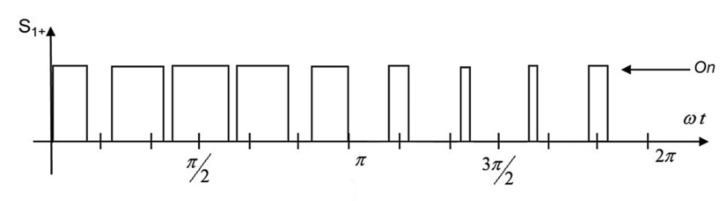
\includegraphics[width=\textwidth]{EMPC_PNG_Pics/CSIwaves_A.png}
                    \caption{\centering The state of switch $S_{1+}$.}
                    \label{BASICCSR:fig:CSIwave_A}
                \end{subfigure}
                ~ %add desired spacing between images, e. g. ~, \quad, \qquad, \hfill etc.
                  %(or a blank line to force the subfigure onto a new line)
                \begin{subfigure}[b]{0.9\textwidth}
                    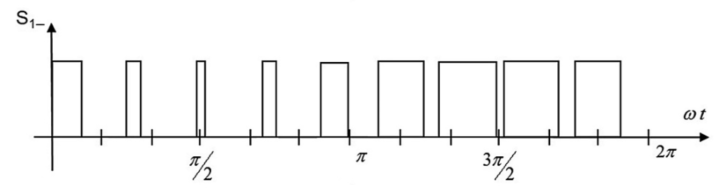
\includegraphics[width=\textwidth]{EMPC_PNG_Pics/CSIwaves_B.png}
                    \caption{\centering The state of switch $S_{2+}$..}
                    \label{BASICCSR:fig:CSIwave_B}
                \end{subfigure}
								 ~ %add desired spacing between images, e. g. ~, \quad, \qquad, \hfill etc.
                  %(or a blank line to force the subfigure onto a new line)
                \begin{subfigure}[b]{0.9\textwidth}
                    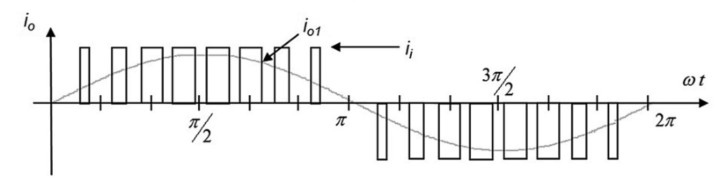
\includegraphics[width=\textwidth]{EMPC_PNG_Pics/CSIwaves_C.png}
                    \caption{\centering AC output current.}
                    \label{BASICCSR:fig:CSIwave_C}
                \end{subfigure}

                \caption{The CSI, ideal waveforms as the result of the modulation.}
                \label{BASICCSR:fig:CSIwave_All}
            \end{figure}

The states for the switches are defined by the modulating technique, which in this case is a carrier-based PWM, but unipolar output is considered. For the CSIs, different output filters may be employed, in order to provide the fundamental component of the output waveform. Depending on the application, it would be desirable to provide a voltage or current output.

\section{Asynchronous parallel pattern search}\label{BASICUNB:sec:APPS}

In the following section, the applied control structure, namely the APPS algorithm shall be discussed in detail. %Optimization (or mathematical optimization) is considered as the mathematical process of finding the best decision for a given problem within a defined set of constraints. In the simplest case, an optimization problem consists of maximizing (or minimizing) a real function by systematically choosing input values from within an allowed input set respective to the given constraints and computing the value of the function. In a controller design case, it deals with the problem of finding the optimal control law for a given system such that a certain optimality criterion is achieved with the best dynamics or lowest amount of energy required.
%The control problem includes a cost functional that is a function of state and control variables. An optimal control is a set of differential equations describing the paths of the control variables that minimize the cost function.
They commonality in this work, is that all of them are designed to search for the optimal control input for a current governing system, should it be voltage unbalance reduction with no applicable network model (due the actors unpredictability), or reaching the fastest reference value with explicit predictive control with the converter's equation's considered, which shall be discussed in section \ref{BASICCSR:sec:MPC}.\\
The APPS can rather be described as a linear search program, distributed in a multi-dimensional plane, where the it is only a black box model available \cite{kolda2003understanding}. These variants of pattern search can solve nonlinear unconstrained problems of the form of:

\begin{equation}
        \begin{array}{c}
            \min_{x\in\mathbb{R}^n}f(x),\\
        \end{array}
        \label{BASICCSR:eqn:currents}
    \end{equation}
		
		where $f:\mathbb{R}^n\longrightarrow\mathbb{R}$. We assume that the evaluation of $f$ is computationally expensive, hence our interest in using either distributed or parallel computing environments to solve the problem. It needs to be concentrated on the parallelization of the search strategy, rather than on the evaluation of $f$, though the techniques we discuss here can be adapted to handle problems for which the computation of $f$ also can be distributed. Additionally is is assumed that $f$ is continuously differentiable. It can be assumed that the gradient $\nabla f$ is unavailable, but the method is applicable as presented in section \oldref{VUB:sec:Optimization}, where the gradient determines the direction of the next step, further increasing its efficiency. For such problems, pattern search methods are one possible solution technique since they neither require nor explicitly estimate derivatives.\\

\myparagraph{Parallel pattern search}

Lets adopt an infinite sequence of iterations $\rho=0,1,2,\dots$, with the last iteration noted as $\rho-1$ and initialization at $0$. It is assumed that the process knows the best point so far as $x^{\rho-1}$, where $f(x^{\rho-1})$ is the global minima of $f$. Associated with $x^{\rho-1}$ there is a step-length control parameter namely $\Delta^{\rho-1}$. Each $i\in\mathcal{P}$, where $\mathcal{P}=\{1,\dots,p\}$ process ends iteration at $\rho-1$ by constructing it's trial point and initiating an evaluation of $f(x^{\rho-1}_i+\Delta^{\rho-1}_id_i)$, where $\mathcal{D}=\{d_1,\dots,d_p\}$ is the finite set of directions applied by each individual process. The simultaneous start of the function evaluations at the trial points on each of the $p$ processes signals the start of iteration $\rho$. When all of the participating processes are finished with their evaluation of $f$, they communicate these values to each other and determine the new values of $x^\rho$, and $\Delta^\rho$. If there exists an $i\in\mathcal{P}$, such that $f(x^{\rho-1}_i+\Delta^{\rho-1}_id_i)<f(x^{\rho-1})$, then $\rho\in\mathcal{S}$, where $\mathcal{S}$ denotes the successful iterations.

\myparagraph{Adding asynchronicity}

 With said above, the general strategy for asynchronous parallel pattern search, from the perspective of a single process $i\in\mathcal{P}$ can be outlined:
		\begin{enumerate}
		\item Evaluate $f(x^{best}_i+\Delta^{best}_id_i)$.
		\item If $f(x^{best}_i+\Delta^{best}_id_i) <f(x^{best}_i)$, then broadcast result to all other processes.
		\item Update local values $x^{best}_i$ and $\Delta^{best}_i$ based on the current local information.
		\item Repeat.
		\end{enumerate}
	The price payed is that each process has its own notion of the best known point seen so far, as well as its own value for	$\Delta^i$. Any success on one process is communicated to all other processes participating in the search, but the successful process carries on from its new best point without waiting for a response from the other processes. By adding a few mild conditions, the global convergence of the search can be still ensured \cite{kolda2003understanding}.  Instead of indexing based on a notion of iterations, we switch from $\rho$ to indexing based on discrete time instance, letting the set $\mathcal{Q}=\{1,2,\dots,q\}$ denote the index of steps. Thus $x_i^q$ s used for the best point known to process $i$ at time step $q$, and similarly, $\Delta_i^q$.  So if process $i$ starts a function evaluation at time step $q$, the trial point at which the function evaluation will be made at $x^{q}_i+\Delta^{q}_id_i$. Further worth mention, that time steps are assumed to be of fine enough resolution so that at most one function evaluation finishes per process per time step.\\
	Lets define two sets that satisfy $\mathcal{Q}=\mathcal{S}_i\cup\mathcal{U}_i$, , and $\mathcal{S}_i=\mathcal{I}_i\cup\mathcal{E}_i$, where $\mathcal{S}_i$ is the set of all time successful steps on process $i$, $\mathcal{I}_i$ is the set if internal successes, $\mathcal{E}_i$ is the set of external successes,   and $\mathcal{U}_i$ consists the unsuccessful steps respectfully. An internal success, where the process finds itself the minima, the external success is where the process is updated externally by the minima. Further  $\mathcal{C}_i\in\mathcal{U}_i$ is defined as the set of time steps where $\Delta^t_i$ is reduced. All the above cases ($\mathcal{U}_i\textbackslash\mathcal{C}_i$) no action is performed.\\
	The updating functions allow us to give the following general definitions for $x_i^q$ and $\Delta^q_i$. For every $q\in\mathcal{Q}$, $q>0$, the best point for the $i^{th}$ process defined to be:
	
	\begin{equation}
        \begin{array}{rcl}
            x_i^q&=&\begin{Bmatrix}
                x_{\omega_i(q)}^{\tau_i(q)}+\Delta_{\omega_i(q)}^{\tau_i(q)}d_{\omega_i(q)},&\textnormal{if }q\in\mathcal{S}_i\\
                x_i^{q-1},&\textnormal{otherwise}\\
            \end{Bmatrix},\\
        \end{array}
        \label{BSIC:equ:APPS_x}
    \end{equation}
		
		with the initialisation $x^0_i=x^0$, where $\omega_i(q)$ is the generating process index for the update time at step $q$ on process $i$, and $\tau_i(q)$ is the time index for initialization of the function evaluation, that produced the update at time $q$ on process $i$. For every $q$ the step length control parameter $\Delta_i^q$ defined to be:
		
		\begin{equation}
        \begin{array}{rcl}
            \Delta_i^q&=&\begin{Bmatrix}
                \lambda_{\omega_i(q)}^{\nu_i(q)}\Delta_{\omega_i(q)}^{\tau_i(q)},&\textnormal{if }q\in\mathcal{S}_i\\
								\theta_{i}^{q}\Delta_{\omega_i(q)}^{\tau_i(q)},&\textnormal{if }q\in\mathcal{C}_i\\
                \Delta_i^{q-1},&\textnormal{otherwise}\\
            \end{Bmatrix},\\
        \end{array}
        \label{BSIC:equ:APPS_Delta}
    \end{equation}
		
		with the initialization $\Delta^0_i=\Delta^0$, where $\nu_i(q)$ is  time index for the completion of the function evaluation that produced the update at time step $q$ on process $i$, and $\theta_i^q$ and $\lambda_i^q$ are chosen. With the following pattern followed, the \hlc[MA]{local} minima of $f$ shall eventually reached \hlc[MA]{with} undetermined steps. 